
\documentclass{article}
\usepackage[utf8]{inputenc}
\usepackage{graphicx}
\usepackage[T1]{fontenc}
\usepackage{lmodern}
\usepackage{listings}
\usepackage[numbers]{natbib} %IEEE
\usepackage{color}
\usepackage{hyperref}
\usepackage{soul}
\usepackage{float}
\usepackage{pgfplotstable}
\usepackage[font=itshape]{quoting}
\usepackage{booktabs}
\usepackage{amsmath}
\usepackage{multicol}
%\usepackage[table,xcdraw]{xcolor}

\usepackage{minted}
\usepackage[a4paper, total={6in, 8in}]{geometry}
\definecolor{dkgreen}{rgb}{0,0.6,0}
\definecolor{gray}{rgb}{0.5,0.5,0.5}
\definecolor{mauve}{rgb}{0.58,0,0.82}
\definecolor{backcolour}{rgb}{0.95,0.95,0.92}
\definecolor{codegreen}{rgb}{0,0.6,0}
% Define a custom style
\lstdefinestyle{myStyle}{
    backgroundcolor=\color{backcolour},   
    commentstyle=\color{codegreen},
    keywordstyle = \bfseries\color{mauve},
    basicstyle=\ttfamily\footnotesize,
    breakatwhitespace=false,         
    breaklines=true,                 
    keepspaces=true,                 
    numbers=left,       
    numbersep=5pt,                  
    showspaces=false,                
    showstringspaces=false,
    showtabs=false,                  
    tabsize=2,
}
\lstset{style=mystyle}

\title{Data Mining \& Machine Learning \\ \large Computer Exercise 5 - Neural Networks \& Backpropagation}
\author{Steinarr Hrafn Höskuldsson}
\date{September 2022}
\newcommand{\mycomment}[1]{}

\begin{document}
\maketitle
\mycomment{
\begin{figure}[h]
    \centering
    \includegraphics[width=0.75\textwidth]{LAB3/Basic1.png}
    \caption{"Switch test" Breadboard set up}
    \label{fig:Switch_test}
\end{figure}

\lstinputlisting[caption=Defining 'ColorMatch' state, label={lst:colormatch}, language=Python, firstline=44, lastline=52]{LAB3/Basic.py}

}
\section*{Section 2.3}

The Neural network was trained using 80\% of the Iris dataset. The accuracy was 96\%, surprisingly good for such a simple model.  The confusion matrix was: 
\\
\begin{center}
CM = 
\begin{bmatrix}
    10 & 0 & 0\\
0 & 9 & 0\\
0 & 2 & 8
    \end{bmatrix}
\end{center}

The misclassification rate and the Average error was plotted as a function of iteration number. The plot can be seen in Figure \ref{fig:section23}. Interestingly, Average error is still trending downwards so it is unclear whether the neural network would improve with more iterations or perhaps overfit.
\begin{figure}[h]
    \centering
    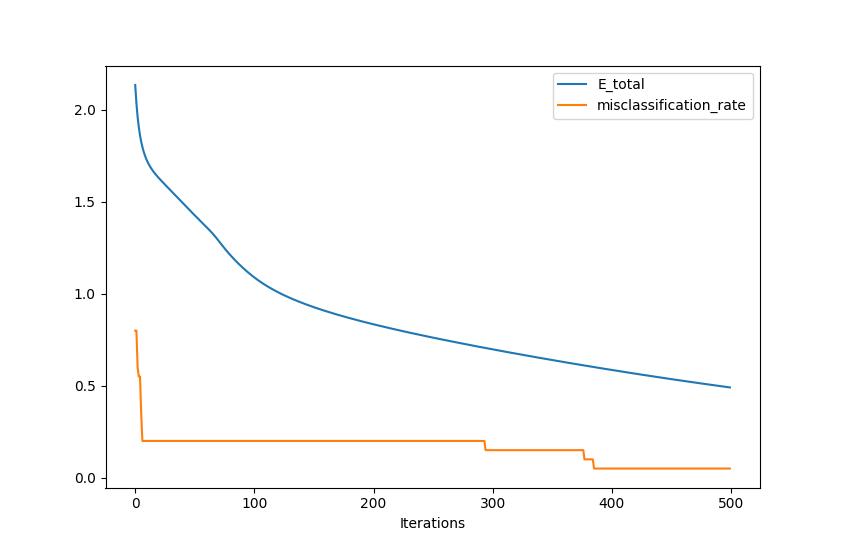
\includegraphics[width=0.75\textwidth]{05_backprop/Section_2_3.png}
    \caption{Average Error and misclassification rate plotted aganist number of iterations}
    \label{fig:section23}
\end{figure}
\section*{Independent}
It might be interesting to investigate what would be a good learning rate (\(\eta\)) for this model and also what might be a good number of iterations(\(N\)). In order to do so a double for loop going though different learning rates and different amounts of iterations was implemented. For each set of learning rate and number of iterations the network was trained and tested on the test set. The resulting accuracies were plotted in pseudocolor plot seen in Figure \ref{fig:indep1}.
%INDEP1.png
\begin{figure}[h]
    \centering
    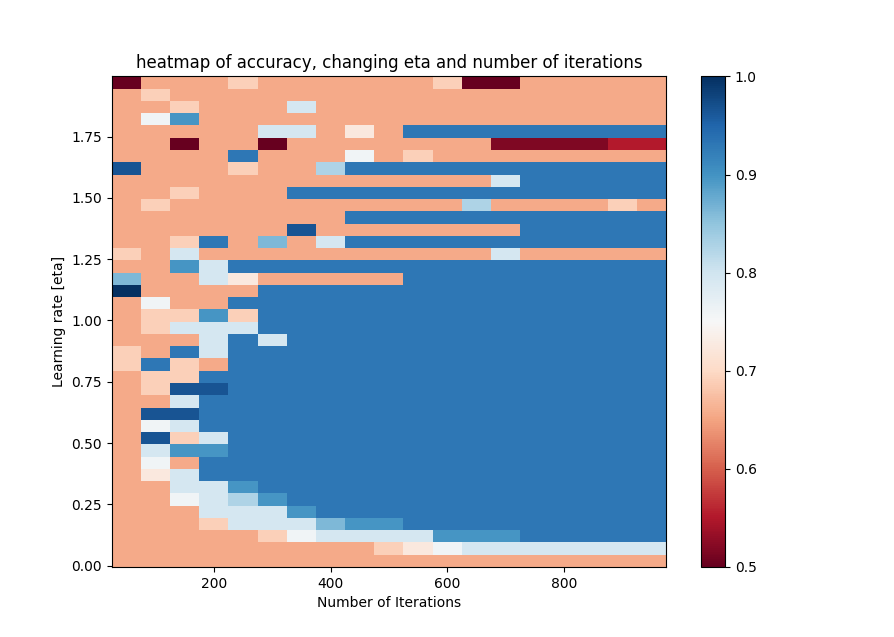
\includegraphics[width=\textwidth]{05_backprop/indep1.png}
    \caption{Heatmap of accuracy, changing \(\eta\) and \(N\)}
    \label{fig:indep1}
\end{figure}
Interestingly, the best result, 100\% accuracy, happens when \(\eta=1.12\) and \(N=50\), It is not because those values somehow match a 'training frequency' causing the network to train very effectively. It is because the test set only has 29 samples. And for this particular split of the dataset, \(\eta=1.12\) and \(N=50\) just happens to get lucky and correctly guess every test sample correctly.

To confirm this, another for loop was implemented and the above calculation was done for 50 different splits of the dataset into test and train samples. The average of the 50 runs were plotted in a pseudocolor plot seen in Figure \ref{fig:indep50} and the Standard deviation of the 50 runs can be seen in Figure \ref{fig:indep50std}
\begin{figure}[H]
    \centering
    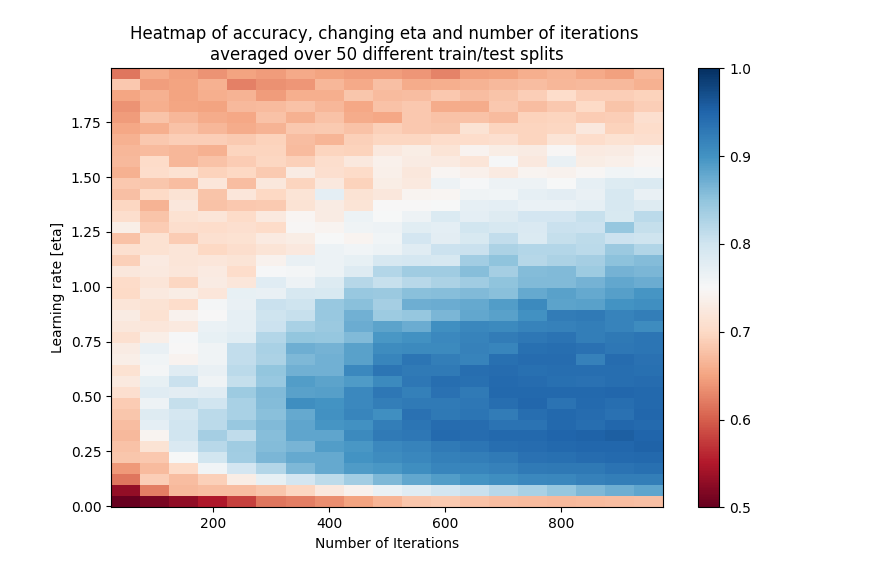
\includegraphics[width=0.9\textwidth]{05_backprop/indep50.png}
    \caption{Heatmap showing average accuracy over 50 runs.}
    \label{fig:indep50}
%\end{figure}
%\begin{figure}[h]
    %\centering
    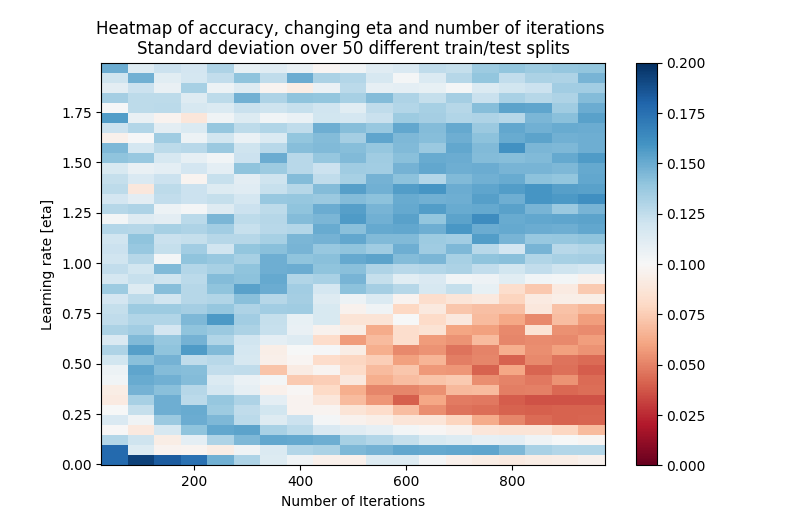
\includegraphics[width=0.9\textwidth]{05_backprop/indep50std.png}
    \caption{Heatmap showing standard deviation of accuracy over 50 runs.}
    \label{fig:indep50std}
\end{figure}

\newpage
It is perhaps more interesting to look at a hybrid of the average and standard deviation, A third plot was made showing the average minus twice the standard deviation. This plot an be seen in Figure \ref{fig:indep50avgstd}. The highest scoring datapoint in the results was ,\(\eta=0.32\) and \(N=900\) with \(avg - 2*std = 0.882\) but an interesting point is ,\(\eta=0.32\) and \(N=600\) with \(avg - 2*std = 0.864\) If we penalize the number of iterations, for example by dividing by \(log(N\) it becomes the highest scoring point. Figure \ref{fig:indep50log} shows \(log(1000)*(avg-2*std)/log(N)\) plotted for the 50 runs.

\begin{figure}[H]
    \centering
    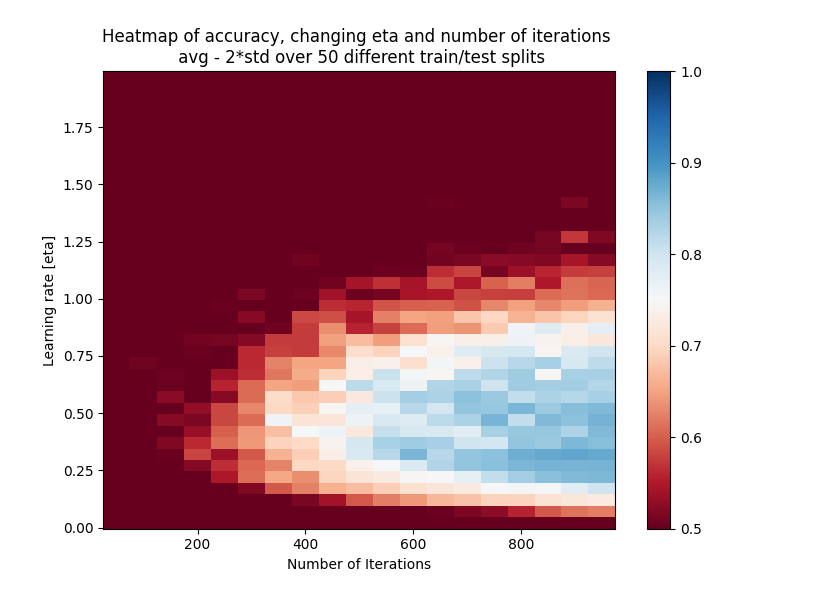
\includegraphics[width=\textwidth]{05_backprop/indep50avgstd.png}
    \caption{Heatmap showing \(avg - 2*std\) of accuracy over 50 runs}
    \label{fig:indep50avgstd}
\end{figure}
\begin{figure}[H]
    \centering
    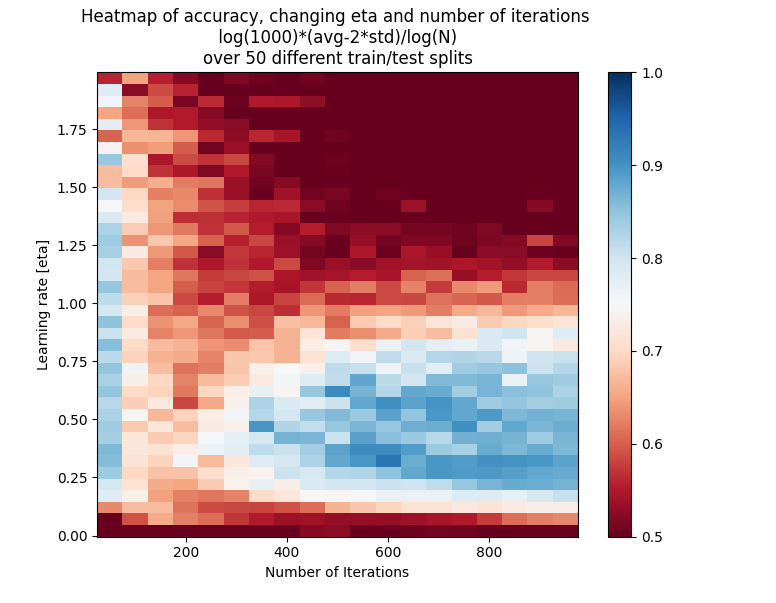
\includegraphics[width=\textwidth]{05_backprop/indep50log.png}
    \caption{Heatmap showing \(log(1000)*(avg-2*std)/log(N)\) over 50 runs}
    \label{fig:indep50log}
\end{figure}
\\

\newpage
\section*{Appendix}
\appendix
\section{Code}

\lstinputlisting[ label={lst:colormatch}, language=Python, ]{05_backprop/Steinarr5.py}


\end{document}

